\documentclass[journal]{IEEEtran}
\IEEEoverridecommandlockouts

\usepackage{cite}
\usepackage{amsmath,amssymb,amsfonts}
\usepackage{graphicx}
\usepackage{textcomp}
\usepackage{xcolor}
\usepackage{tabularx}
\usepackage{booktabs}
\usepackage{array}
\usepackage[colorlinks,linkcolor=red,anchorcolor=red,citecolor=blue,urlcolor=blue]{hyperref}
\usepackage{tikz}
\usetikzlibrary{arrows.meta, positioning, shapes.geometric, fit, backgrounds, calc}

\graphicspath{{./figs/}}

\definecolor{paperBlue}{RGB}{35,79,140}
\definecolor{paperGreen}{RGB}{34,125,92}
\definecolor{paperGold}{RGB}{176,125,33}
\definecolor{paperRed}{RGB}{178,72,72}
\definecolor{paperSoft}{RGB}{246,248,250}
\definecolor{paperLine}{RGB}{80,92,110}

\newcommand{\artifact}{\texttt{ArtifactSeries}}
\newcommand{\versionrecord}{\texttt{VersionRecord}}
\newcommand{\typer}{\texttt{TypeRegistry}}
\newcommand{\typeindex}{\texttt{TypeIndex}}
\newcommand{\commentstree}{\texttt{CommentsTree}}
\newcommand{\likesbook}{\texttt{LikesBook}}
\newcommand{\pprf}{\texttt{PPRF}}
\newcommand{\BibTeX}{\rm B\kern-.05em{\sc i\kern-.025em b}\kern-.08em
    T\kern-.1667em\lower.7ex\hbox{E}\kern-.125emX}

\begin{document}

\title{PaperProof: Sui-Native Artifact Infrastructure for Durable, Verifiable, and Agent-Readable Knowledge Objects}

\author{\IEEEauthorblockN{PaperProof Labs}\\
\IEEEauthorblockA{\href{mailto:paperproof.labs@gmail.com}{paperproof.labs@gmail.com}\\
\href{https://paperproof.site/}{https://paperproof.site/}\\
\href{https://github.com/PaperProofLabs}{https://github.com/PaperProofLabs}}}

\maketitle

\begin{abstract}
Important digital works increasingly live across unstable boundaries: storage links, social feeds, repository releases, preprint pages, chat archives, and application databases. These surfaces are useful, but none of them alone provides a neutral and composable protocol identity for the work itself. PaperProof is a Sui-native protocol for durable, verifiable, and community-governed artifacts backed by Walrus content storage. It treats a work not as a single uploaded file, but as a continuing artifact series with typed versions, content commitments, official interaction objects, governance-aware parameters, and canonical events that can be consumed by applications, SDKs, indexers, and agentic interfaces.

This paper presents PaperProof as artifact infrastructure rather than as a narrow publishing website. The protocol separates compact state from large content: Sui stores artifact identity, type state, version records, comments, likes, governance, fee configuration, prompt and memory capability registries, and events, while Walrus stores large content such as PDFs, datasets, source archives, software packages, images, long-form text, and prompt packages. The first official application remains a static wallet-bounded web app, while a reference indexer now supplies server-assisted views and verified public-content caches for faster reads. Developer access is provided through role-specific TypeScript, Python, and Rust SDKs for frontend integration, scripting and analytics, and high-performance indexing.

We describe the protocol model, on-chain object architecture, content binding, query and watch semantics, governance path, SDK ecosystem, and a browser-side agentic interface called PaperProof Copilot. Copilot uses protocol-native prompts stored as PaperProof artifacts and an optional wallet-linked memory layer whose public registry records only discovery and availability metadata while private memory remains outside PaperProof chain state. The design goal is not to replace academic archives, social platforms, repositories, or storage networks. Instead, PaperProof supplies a durable layer beneath and beside them: a verifiable identity and event surface for artifacts that should remain interpretable across frontends, market cycles, and organizational changes.
\end{abstract}

\begin{IEEEkeywords}
artifact infrastructure, Sui, Walrus, decentralized storage, protocol identity, indexers, SDKs, agentic interfaces, governance
\end{IEEEkeywords}

\section{Introduction}

Digital knowledge is not only published; it is revised, mirrored, discussed, indexed, summarized, cited, packaged, and rediscovered. A preprint may point to a dataset, a dataset may depend on source code, a software release may carry a changelog, and a community may later debate which version should be considered canonical. The objects that matter are no longer only papers. They are durable digital artifacts.

Yet most artifacts still depend on application-specific records for their public life. A repository release is tied to a hosting provider. A preprint page is tied to an archive. A long-form post is tied to a website or social platform. A dataset may be copied across storage systems without preserving a shared interaction and governance history. Content hashes help, but a hash alone does not express artifact type, version lineage, owner, official comments, governance state, or which event stream indexers should trust.

PaperProof addresses this missing layer. It defines a Sui-native artifact protocol in which a work receives a durable protocol identity, evolves through typed versions, binds to Walrus content, emits canonical events, and exposes official interaction objects. The protocol is intentionally not a full social network, repository host, peer-review system, or recommendation engine. It is a smaller substrate: a way to make important digital works verifiable, composable, indexable, and agent-readable.

\begin{figure*}[!t]
    \centering
    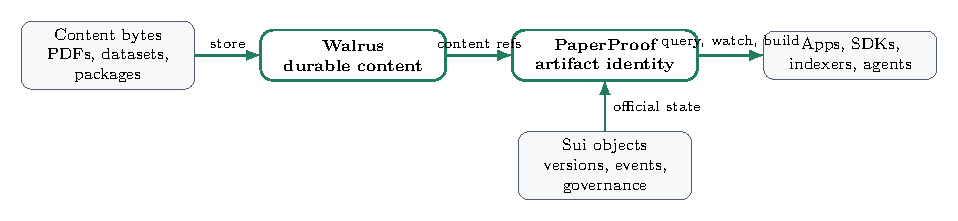
\includegraphics[width=0.95\textwidth]{core-model.pdf}
    \caption{PaperProof turns content stored on Walrus into Sui-native protocol artifacts with typed versions, official interactions, governance, and developer-facing query surfaces.}
    \label{fig:core_model}
\end{figure*}

The current implementation trajectory is deliberately product-oriented. PaperProof includes mainnet contracts, a static official web application, deployment manifests, SDKs in TypeScript, Python, and Rust, optional mainnet integration harnesses, and a browser-side Copilot that explains protocol state while preserving wallet approval boundaries. These components are not peripheral. They are part of the argument: a protocol for long-lived artifacts must be usable by ordinary applications and robust enough for indexers and automation.

This paper makes four contributions. First, it proposes an artifact-series model for durable works that can evolve through typed versions. Second, it describes a Sui/Walrus architecture that separates protocol state from large content without reducing artifacts to bare storage links. Third, it presents an SDK and indexer surface that treats events, deployment manifests, and query providers as first-class protocol integration concerns. Fourth, it introduces a human-approved agentic interface pattern in which AI can interpret artifact state, retrieve protocol-native prompts, and use optional wallet-linked memory without controlling keys or signing transactions.

\subsection{Problem Statement}

PaperProof targets the following systems problem: given a digital work whose bytes may live in decentralized storage and whose social life may span many applications, how can a public protocol assign a durable identity, preserve typed version history, bind verifiable content references, expose official interactions, and allow independent applications to reconstruct the same state without trusting one website or database?

This problem has three constraints. First, the protocol must not put large content on chain. Second, it must not require every frontend or indexer to understand low-level Move internals before it can show a correct view. Third, it must remain upgradeable enough for an early protocol while giving integrators a stable way to discover the active deployment. PaperProof's design choices follow from these constraints.

\section{Background and Motivation}

\subsection{Artifacts Beyond Files}

The word artifact is deliberately broader than file. A file is a byte sequence. An artifact is a work with identity, context, authorship, history, interpretation, and social use. A preprint is not only a PDF; it has authors, abstract, topic, license, and version lineage. A dataset is not only an archive; it has format, schema, provenance notes, and often a relationship to papers or software. A software release is not only a tarball; it has source references, package hashes, changelogs, and compatibility expectations. A long-form protocol post is not only text; it may become part of a community's institutional memory.

Most digital infrastructure handles files well but handles artifacts indirectly. Storage systems can preserve bytes. Social platforms can amplify links. Code hosts can present releases. Academic archives can show paper pages. These systems are valuable, but each keeps its own model of identity and interaction. When an artifact moves across systems, its public life fragments. One application may know the versions; another may know comments; another may hold the bytes; another may provide a citation link. The artifact itself does not have a neutral protocol coordinate.

PaperProof is motivated by this gap. It does not try to replace the specialized platforms that surround artifacts. Instead, it gives artifacts a protocol-level identity and lifecycle that multiple platforms can read. The intention is closer to a durable coordinate system than to a monolithic application.

\subsection{Limits of Hash-Only Provenance}

Content hashes are necessary but not sufficient. A hash can identify a byte sequence, but it cannot say what type of artifact the bytes represent, whether the artifact is the first version or a later version, who published it through the protocol, whether it has official comments, which likes book belongs to it, whether a governance proposal affected its fees or type status, or whether an event came from the current official deployment.

Hash-only provenance also makes user experience brittle. A normal user does not want to compare long digests as the primary way to navigate knowledge objects. Applications need typed metadata, stable display codes, ownership, timestamps, content types, version numbers, and relationships. Indexers need canonical event filters and object bindings. Agents need structured state that can be explained. PaperProof treats hashes as part of the binding, not as the entire identity model.

\subsection{Why Application Databases Are Not Enough}

A conventional web application can implement nearly every feature of PaperProof in a private database: uploads, versions, comments, likes, governance-like polls, and search. The issue is not feasibility. The issue is authority. If one database is the ultimate source of artifact existence and interaction history, then other applications remain downstream of that operator. If the operator disappears, changes policy, loses data, or silently rewrites records, the public artifact history becomes difficult to reconstruct.

Blockchains do not remove all trust, but they change where trust is placed. Prior work has explored blockchain-mediated scholarly publishing, smart papers, decentralized peer review, open science infrastructure, cooperative scholarly communication, and broader DeSci values \cite{hoffman2019scholarly,tenorio2021decentralizing,stojmenova2019publish,janowicz2018prospects,weidener2024desci,hoffman2020decentralization}. PaperProof builds on that motivation but focuses on a narrower infrastructure question: how to represent many kinds of durable artifacts, not only scholarly papers, as protocol objects with typed versions and official interaction surfaces. It places compact authoritative state and event history in Sui objects, while large content remains in Walrus. The official frontend becomes an access layer rather than the sole source of truth. This is especially important for a protocol that aims to support community portals, indexers, academic tools, AI workflows, and future frontends that may not exist at the time an artifact is published.

\subsection{Design Opportunity in Sui and Walrus}

Sui and Walrus create a practical opening for this design. Sui's object model and the Move resource model make it natural to represent protocol objects directly rather than simulating object relationships through account-keyed maps \cite{mysten2022sui,welc2023sui_move,blackshear2020move,sui_docs}. Walrus provides a storage layer for large content and a deployment target for static applications \cite{danezis2025walrus,walrus_docs}. The result is a stack in which a protocol can be public and object-oriented without forcing every artifact byte on chain or every application through one hosted backend.

PaperProof therefore starts from a product-level observation: if Sui transactions are cheap enough and Walrus content operations are usable enough, then artifact interactions can be normal actions rather than rare ceremonial registrations. Publishing, adding versions, commenting, liking, voting, claiming, and maintaining content can become part of a living protocol workflow.

\subsection{The Missing-Layer Hypothesis}

Sui supplies programmable objects and Walrus supplies durable content, but neither layer alone defines the public life of a knowledge artifact. A stored blob does not specify its continuing identity, typed lineage, official interactions, governed agent prompt, or canonical event surface. An application database can add these features, but then the application becomes the authority. PaperProof tests a missing-layer hypothesis: artifact identity and agent-readable context should be protocol infrastructure that multiple applications can reconstruct independently.

This hypothesis shifts the evaluation question. The relevant question is not whether bytes can be uploaded to decentralized storage. It is whether stored content can become a verifiable, versioned, discussable, indexable, and agent-readable object without forcing every future client to trust one hosted service.

\section{Design Goals and Non-Goals}

PaperProof is shaped by a narrow principle: the protocol should record durable artifact facts, not replace every platform that surrounds an artifact.

\subsection{Design Goals}

The first goal is durable identity. A PaperProof artifact should have a stable series identity that survives a particular frontend, website, social post, or repository page. The human-readable artifact code is useful for display, but the authoritative identity is the Sui object binding under the official protocol root.

The second goal is typed evolution. A continuing work should evolve through append-only versions. A preprint, dataset, software release, blog post, technical report, or generic file should not all be forced into one untyped blob record. Type-specific fields make applications safer and indexers more useful.

The third goal is verifiable content binding. Sui should not store large files, but it should store enough information to identify and verify the content held by Walrus. Content hashes, blob identifiers, blob object identifiers, content types, and version records form the bridge between state and storage.

The fourth goal is official interaction binding. Comments and likes are not merely frontend decorations. Each artifact series has official interaction objects so that applications can identify the comments and signals that belong to the artifact through trusted object relationships.

The fifth goal is integration reliability. A protocol that expects third-party use must offer more than raw Move calls. PaperProof provides SDKs, typed builders, deployment manifests, query providers, watch APIs, event filters, and indexer-oriented primitives to reduce integration mistakes.

The sixth goal is low-maintenance survival. The first official application is static and can be deployed through Walrus Sites. The protocol should remain legible even if the initial application layer is quiet for long periods. Rich search, moderation, analytics, and portals can grow above the durable core.

The seventh goal is multi-surface usability. PaperProof is expected to be used from a browser wallet, a Node.js script, a Python notebook, a command-line export tool, a Rust indexer, a static site, or an AI assistant. The protocol should not assume that one frontend is the only meaningful client. This is why the SDKs are not treated as afterthoughts.

The eighth goal is honest degradation. Web3 applications often present incomplete data as if it were complete. PaperProof should make it easier for clients to distinguish empty state from failed reads, old package events from current package events, and provider limitations from protocol facts.

\subsection{Non-Goals}

PaperProof does not judge truth, originality, scientific quality, license compliance, or social value. It can prove that an address committed to typed metadata and content references through an official protocol path. It cannot prove that the content is correct or worthy.

PaperProof does not attempt to be a social network, repository host, issue tracker, full-text search engine, review platform, or recommendation algorithm. Those are application-layer responsibilities. The protocol supplies facts that such systems can interpret.

PaperProof also does not aim for irreversible ossification at launch. Early protocols need upgrade paths for security fixes, new artifact types, SDK alignment, and governance improvements. The design therefore treats deployment manifests, drift checks, and governance-controlled activation as part of operational safety.

\subsection{Protocol Invariants}

The system is designed around a small set of invariants that applications and indexers can rely on.

\begin{itemize}
    \item An artifact series has exactly one protocol-recognized artifact type and one human-readable artifact code.
    \item A version belongs to one series, has one version number, and does not mutate prior version records.
    \item Official comments and likes are valid only through the interaction objects bound to the series.
    \item Event streams are not self-authenticating; they must be interpreted under the active package, root, and object bindings.
    \item Large content is external to Sui object state, but content references and verification material are part of version state.
    \item SDKs may simplify workflows, but signing authority remains with the user wallet, keypair, or execution provider.
\end{itemize}

These invariants keep PaperProof smaller than a full content platform while giving third parties enough structure to build reliable applications.

\subsection{Design Principles}

The first design principle is series-first identity. A continuing work should not be modeled as an isolated upload. It should have a stable series object that can accumulate versions, comments, likes, and governance-relevant interpretation over time. This gives applications one durable place to start when resolving an artifact.

The second principle is typed minimalism. Artifact types should be expressive enough to prevent every work from becoming an opaque blob, but scarce enough that the protocol does not become a schema registry for arbitrary application data. The six initial types provide practical coverage while leaving room for governance-controlled expansion.

The third principle is official interaction binding. PaperProof does not try to prevent every unofficial comment, mirror, or like from existing elsewhere. Instead, it defines which interaction objects are official for a series. This is a more realistic standard than attempting to control all social activity around an artifact.

The fourth principle is layered authority. Sui objects define official state. Walrus carries large content. SDKs encode common integration rules. Indexers derive queryable views. Applications and agents explain and present the result. Each layer has a job; none should pretend to replace all the others.

The fifth principle is wallet-bounded automation. Builders, services, and agents can reduce user burden, but transaction approval remains at the wallet or signer boundary. This is especially important when AI assistance is present. The system should make the next action understandable without silently taking authority from the user.

The sixth principle is workflow composition. Sui Programmable Transaction Blocks (PTBs) can group compatible Move calls into one user-signable action. PaperProof can use PTBs to reduce signature burden for publication, versioning, comments, registry updates, and related flows while still respecting external storage phases such as Walrus reserve and certify operations. This matters because a technically composable protocol can still fail at the product layer if users must approve a confusing sequence of low-level calls.

\section{Layered Architecture}

PaperProof consists of six cooperating layers: content, protocol state, events, query/indexing, applications, and agentic assistance. Fig.~\ref{fig:architecture} summarizes the intended formal release architecture.

\begin{figure*}[!t]
    \centering
    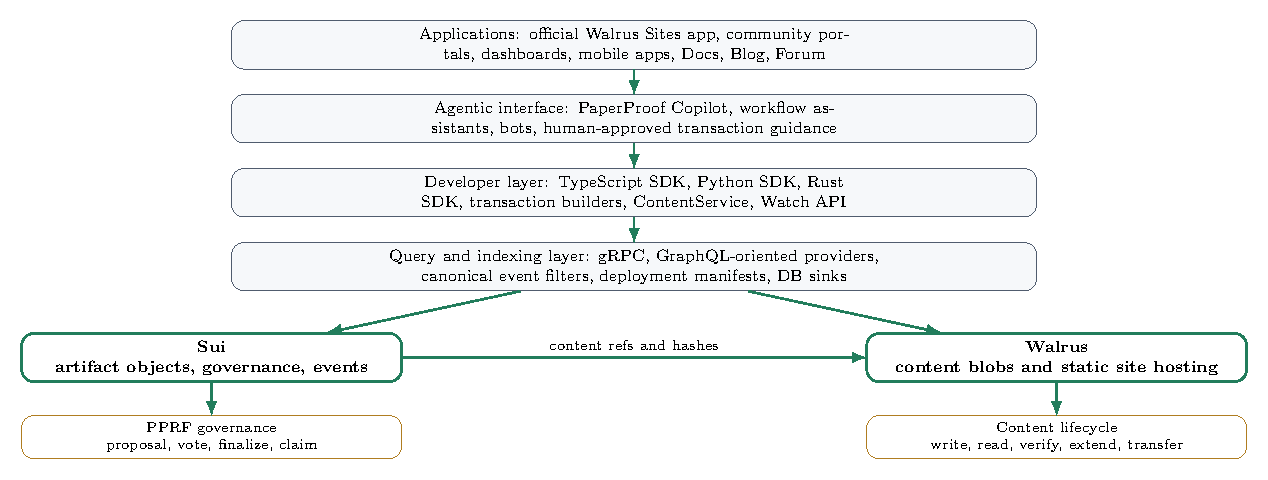
\includegraphics[width=\textwidth]{release-architecture.pdf}
    \caption{PaperProof release architecture. The protocol core is small, while applications, SDKs, indexers, and agentic workflows can evolve around the same Sui and Walrus foundation.}
    \label{fig:architecture}
\end{figure*}

\begin{figure*}[!t]
    \centering
    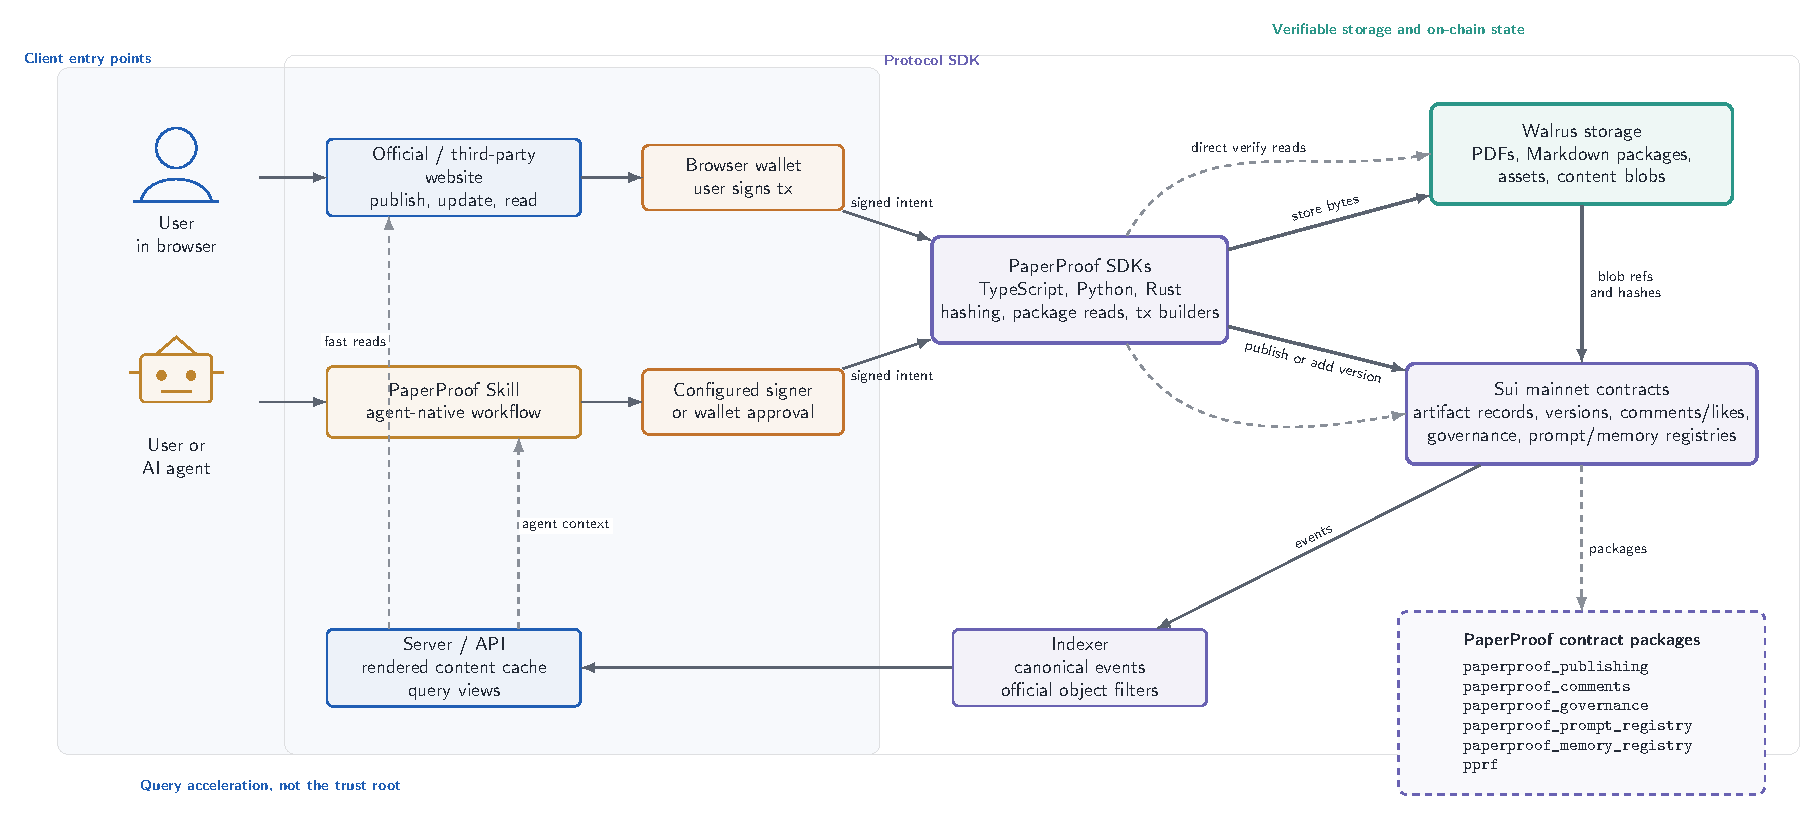
\includegraphics[width=0.92\textwidth]{application-architecture-flow.pdf}
    \caption{PaperProof application architecture and workflow. Human users and AI agents can enter through official or third-party websites and the PaperProof Skill; the shared execution path binds Sui mainnet contracts, Walrus storage, server-side indexing, and SDK access into one artifact protocol surface.}
    \label{fig:application_architecture_flow}
\end{figure*}

\subsection{Content Layer}

The content layer is carried by Walrus. It stores large blobs: PDFs, datasets, source archives, software packages, images, long comments, and other content that should not become Sui object bytes. PaperProof records Walrus references and content commitments so that applications can retrieve and verify the corresponding content. This places PaperProof in the broader family of content-addressed and decentralized storage designs represented by IPFS, Filecoin, and Arweave \cite{benet2014ipfs,protocol_labs2017filecoin,williams2023arweave}, while using Walrus as the storage substrate that is native to the target deployment stack \cite{danezis2025walrus,walrus_docs}.

PaperProof SDKs include a ContentService abstraction so users do not need to treat Walrus as a separate toolchain for common flows. The service can publish content, read it, verify digests, extend storage, and transfer owned blobs where allowed. Shared and owned blob semantics are surfaced because extending or transferring content has different preconditions.

\subsection{Protocol State Layer}

The state layer is carried by Sui Move contracts. It records artifact identity, type activation, version records, official comment and like objects, fee configuration, governance state, proposal lifecycle, votes, claims, and canonical events. This layer answers what PaperProof recognizes as official.

Sui is well matched to this role because PaperProof is object-centric. Artifact series, typed versions, comments trees, likes books, governance vaults, and fee managers are not rows in a private database. They are protocol objects with explicit relationships.

\subsection{Event and Query Layer}

Events are the bridge from on-chain state to applications and indexers. PaperProof emits events for publication, versioning, metadata updates, ownership transfer, comments, likes, governance proposals, voting, finalization, claims, fee changes, and upgrade-adjacent operations. Events are evidence, not conclusions. Applications should filter events through official package IDs, root bindings, and object relationships before using them as facts.

The query layer is intentionally provider-based. Sui's JSON-RPC sunset path makes it unsafe for SDKs to hardcode one historical query mechanism. PaperProof therefore treats gRPC, GraphQL-oriented event retrieval, deployment manifests, and indexer-specific sinks as replaceable provider surfaces.

\subsection{Application Layer}

The first official application is a static PaperProof web app rather than a server-owned platform. Its pages map directly to protocol concepts. Explore presents recent artifacts by type and opens detailed artifact pages. Publish guides users through type-specific publication. Governance exposes active proposals, voting history, and claimable funds. My Space shows wallet state, personal artifacts, and voting records. Docs, Blog, and Forum are application surfaces that can themselves be backed by protocol artifacts rather than by a private content database.

\begin{figure}[!t]
    \centering
    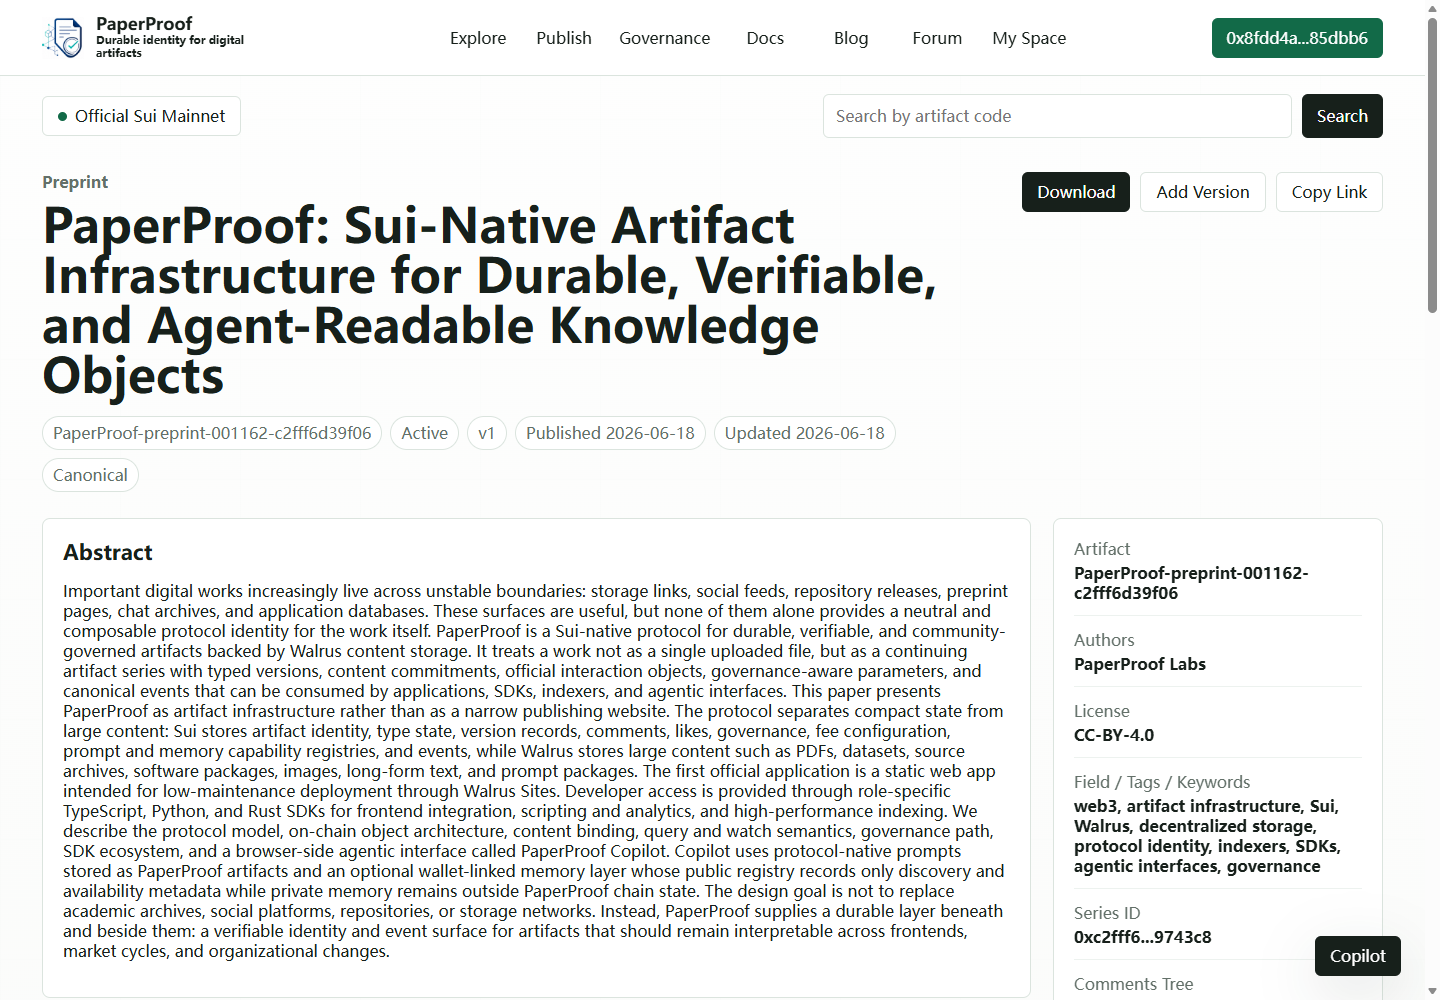
\includegraphics[width=\columnwidth]{official-preprint-detail.png}
    \caption{An official preprint detail view. The page is an application rendering of protocol facts: artifact code, series and version IDs, content hash, Walrus references, authorship metadata, and version history.}
    \label{fig:official_preprint_detail}
\end{figure}

This application is official, but it is not exclusive. A university archive, a research-group portal, a software release dashboard, a mobile app, a community forum, or an autonomous indexing service can all use the same protocol objects. PaperProof's goal is therefore not to trap users inside one frontend. It is to make the protocol facts sufficiently typed and discoverable that multiple frontends can coexist.

The application layer may also make policy choices that are intentionally not global protocol mutations. An official frontend may hide, de-rank, label, or refuse to preview content because of abuse, legal risk, provider failure, or product policy. Such non-display does not erase Sui records or decentralized-storage content. This separation is a practical consequence of combining durable infrastructure with independently operated presentation layers.

\section{Why Sui and Walrus Are Structural}

PaperProof depends on two properties that are difficult to reproduce with a conventional chain-plus-server design: cheap object-centric state transitions and durable programmable content storage. The first property follows from Sui's object-centric smart-contract platform \cite{mysten2022sui,sui_docs} and Sui Move's object-oriented programming model \cite{welc2023sui_move,blackshear2020move}. The second follows from decentralized storage systems that decouple content persistence from a single web host \cite{benet2014ipfs,protocol_labs2017filecoin,williams2023arweave,danezis2025walrus,walrus_docs}.

Sui contributes the object model. PaperProof's core entities are naturally objects: a root, a type registry, type indexes, artifact series, typed version records, comment trees, likes books, a governance vault, proposals, votes, claims, and fee configuration. Object ownership and shared-object access map cleanly to publication ownership, official interaction objects, and governance-controlled mutation. Low transaction costs also matter. Comments, likes, version additions, and governance interactions should not feel like rare ceremonial actions; they should be ordinary protocol operations.

Walrus contributes the content layer. Storing large PDFs, datasets, archives, and long-form text directly on chain would be economically and technically inappropriate. Storing them only on a centralized server would weaken the protocol's survival story. Walrus lets PaperProof bind large content to compact on-chain facts while still supporting static application deployment through Walrus Sites.

The combination is what makes PaperProof plausible as a long-lived artifact protocol. Sui records the official state transitions; Walrus carries the large content and public application surface; SDKs and indexers connect both layers into usable workflows. Without Sui's object model, artifact relationships would be harder to express safely. Without Walrus, PaperProof would collapse into either a link registry or a conventional website with a chain receipt.

\section{On-Chain Object Model}

The protocol object model is summarized in Fig.~\ref{fig:object_model}. The figure uses a dashed node for the logical type entry because \typer{} stores enabled \texttt{TypeInfo} records and \typeindex{} object IDs, while \artifact{} objects are discovered through events and their own artifact type fields rather than being directly owned by the registry.

\begin{figure*}[!t]
    \centering
    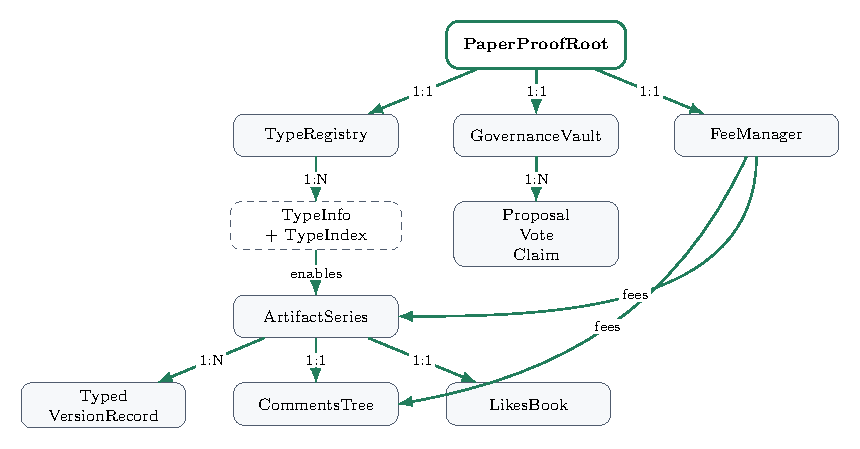
\includegraphics[width=0.95\textwidth]{on-chain-object-model.pdf}
    \caption{PaperProof on-chain object model. The registry controls type recognition; artifact series and their official interaction objects form the durable identity surface.}
    \label{fig:object_model}
\end{figure*}

\subsection{Root, Type Registry, and Type Indexes}

\texttt{PaperProofRoot} is the trust anchor. It records the official governance vault, fee manager, type registry, and internal capabilities used by official publishing and governance paths. Frontends and indexers should begin trust evaluation from this root rather than by accepting any object with a matching Move type.

\typer{} records protocol-recognized artifact types, enabled state, schema version, minimum protocol version, and \typeindex{} object IDs. Built-in types include \texttt{preprint}, \texttt{blog\_post}, \texttt{technical\_report}, \texttt{dataset}, \texttt{software\_release}, and \texttt{generic\_file}. The type set is intentionally scarce. Adding a new protocol-recognized type requires contract support, SDK builders, views, validators, event parsing, documentation, tests, and governance activation.

\begin{table*}[!t]
\centering
\caption{Built-in artifact types and their intended first-class semantics.}
\label{tab:artifact_types}
\begin{tabularx}{\textwidth}{>{\raggedright\arraybackslash}p{3cm}>{\raggedright\arraybackslash}p{4.4cm}>{\raggedright\arraybackslash}X}
\toprule
Artifact type & Typical content & Protocol-level reason for a distinct type \\
\midrule
\texttt{preprint} & Manuscripts, abstracts, author lists, fields, licenses & Preserves scholarly-version lineage and makes citation-oriented applications easier to build. \\
\texttt{blog\_post} & Official posts, community essays, release notes, protocol narratives & Allows durable long-form content without turning the protocol into a centralized blog host. \\
\texttt{technical\_report} & Specifications, audits, design notes, engineering reports & Gives formal technical documents a versioned identity outside short-lived repositories. \\
\texttt{dataset} & Data archives, schemas, checksums, collection notes & Separates dataset-specific metadata from generic file upload semantics. \\
\texttt{software\_release} & Source archives, binary packages, package hashes, changelogs & Supports software supply-chain records and reproducible release references. \\
\texttt{generic\_file} & Miscellaneous files, bundles, media, compressed archives & Provides an escape hatch for useful artifacts that do not yet justify a protocol type. \\
\bottomrule
\end{tabularx}
\end{table*}

\subsection{Artifact Series and Typed Versions}

\artifact{} is the stable identity of a continuing work. It stores artifact type, artifact code, owner, current version number, current version ID, version IDs, official comments tree ID, official likes book ID, status, metadata extensions, and timestamps.

A version record is an immutable typed snapshot under a series. All versions share a common header: series ID, artifact type, version number, previous version ID, author, content hash, Walrus blob ID, Walrus blob object ID, content type, status, timestamp, and bounded metadata extensions. Each artifact type adds fields that matter for that type. A dataset needs format and size semantics; a software release needs source and package hash semantics; a preprint needs title, abstract, authors, field, and license semantics.

The separation between series state and version state is deliberate. Series state answers ``what is the continuing work and where is its current head?'' Version state answers ``what exact content and typed metadata were committed at this point in the work's history?'' Applications can therefore show a convenient latest view without losing historical verifiability. Indexers can rebuild both views: a latest-state table for browsing and an append-only version table for audit.

\subsection{Typed Views}

PaperProof exposes typed views above raw object fields. A typed view normalizes object IDs, owner addresses, version numbers, timestamps, content references, status fields, and type-specific metadata into stable SDK-level structures. This reduces the amount of Sui-specific detail a normal application must handle. At the same time, advanced users can still access raw object data when they need a lower-level integration.

Typed views also protect against partial data. For example, an artifact detail page may have the series object but temporarily fail to load the comments tree. In that case the correct state is not ``zero comments''; it is ``series loaded, comment view degraded''. View construction should preserve that distinction so interfaces can be honest about what they know.

\subsection{Official Comments and Likes}

Each series receives official interaction objects. \commentstree{} is the official threaded discussion object for an artifact. It supports short on-chain comments and blob-backed longer comments, enforces depth and content limits, and binds to the correct series, root, governance vault, and fee manager. \likesbook{} records like state separately from comments, reducing shared-object contention and making lightweight signals easier to index.

These objects matter because decentralized applications often misinterpret raw events. A comment event is not necessarily an official artifact comment unless its tree is bound to the official series. A like event is not necessarily a valid protocol signal unless its likes book is the one bound to the artifact.

\subsection{Governance and Fees}

\texttt{GovernanceVault} records protocol authority boundaries, proposal state, voting, claims, executable governance action support, and direct authority modes. \texttt{FeeManager} stores fee levels for artifact types and comments under the official root. The design keeps operational recovery possible during early stages while creating a path toward stronger PPRF-governed control.

\subsection{Identifier and Discovery Model}

PaperProof separates display identifiers from authority. The artifact code is meant to be human-readable and searchable. It helps users communicate about an artifact without copying an object ID. However, the object ID of the \artifact{} and its binding under the active root remain the authoritative identity. This distinction lets the protocol support friendly codes while preventing applications from trusting a string alone.

Discovery is event-assisted rather than registry-owned. The type registry recognizes types and type indexes, but it does not directly own every artifact series. Indexers discover series through canonical publication events and validate them through object reads and root/type relationships. This avoids forcing all artifact discovery through one ever-growing registry object while still giving applications a way to rebuild type-specific views.

\subsection{Status and Metadata Model}

Status fields are intended to be protocol facts, not editorial judgments. A status can help applications understand whether a version or series is active, hidden, deprecated, or otherwise marked by a supported workflow. It should not be confused with truth, quality, peer review, or endorsement.

Metadata extensions provide controlled flexibility. They let applications attach bounded key-value style information that is not yet important enough to become a first-class Move field. The SDK validates duplicate keys, size limits, and normal forms so metadata remains useful for indexing. When a metadata pattern becomes important across many applications, it can be promoted into a type-specific field through a future type/schema update.

\subsection{Ownership and Authority Model}

Ownership in PaperProof is not one-dimensional. A user may own a series, another object may hold a content blob, governance may control fee parameters, and a wallet may approve a transaction built by an application. The protocol therefore distinguishes artifact ownership, content ownership, governance authority, execution authority, and display authority.

This distinction is especially important for frontends. A connected wallet may be able to comment but not add a version. It may be able to vote but not execute a proposal. It may have locked funds that can be claimed only after finalization. A good SDK should expose these differences as typed state rather than making the frontend infer them from low-level failures.

\section{Artifact Lifecycle}

PaperProof models artifact publication as a versioned protocol lifecycle rather than a single upload. Fig.~\ref{fig:lifecycle} shows the core path.

\begin{figure*}[!t]
    \centering
    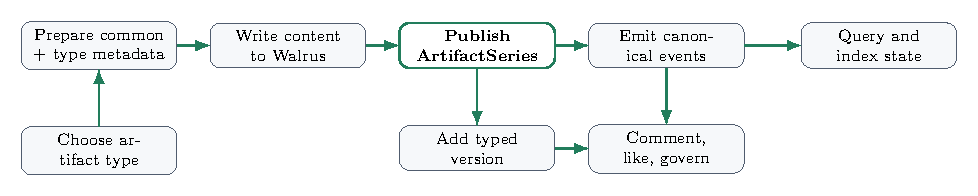
\includegraphics[width=\textwidth]{artifact-lifecycle.pdf}
    \caption{Artifact lifecycle. Publication creates a series and first typed version; later versions, comments, likes, and governance actions extend the protocol life of the artifact.}
    \label{fig:lifecycle}
\end{figure*}

\subsection{Publishing}

Publishing begins with type selection. The common fields identify content hash, Walrus references, content type, metadata extensions, and fee payment. Type-specific fields provide structured semantics. The SDK validates empty titles, invalid object IDs, duplicate metadata keys, oversized fields, and other errors before the wallet signs.

The publish transaction creates an \artifact{}, a first typed version record, a \commentstree{}, and a \likesbook{}. It emits events that indexers can use to reconstruct discovery state. The artifact code is human-readable, but the series object ID and official root binding remain authoritative.

The publishing path intentionally separates preparation from authorization. A frontend or script may compute content hashes, upload to Walrus, prepare metadata, and build a transaction before the wallet signs. None of these steps alone creates a protocol artifact. The artifact exists only after the official publish transaction succeeds under the active deployment.

This separation matters for failure recovery. A Walrus upload may succeed while the Sui transaction fails. A wallet may reject the transaction after content preparation. A frontend may lose local state after building the transaction. The SDK should therefore return structured intermediate data and typed execution results so users can understand which stage completed and which did not.

\subsection{Adding Versions}

Adding a version is a continuation of an existing series. Some fields are immutable at the series level, such as artifact type and code. The Add Version page in the official app therefore uses a subset of the Publish fields while displaying immutable series context. The resulting version is append-only: previous versions remain available for verification and interpretation.

Version addition uses the same content-binding pattern as initial publication, but it is stricter in what it allows to change. A new version may replace content, update type-specific fields, add metadata, or change status-like information according to the type rules. It may not transform a preprint into a dataset or rewrite the artifact code. This keeps the series meaningful over time.

The version chain also gives applications a natural comparison surface. A reader can see whether a dataset changed format, whether a software release changed package hash, whether a technical report revised its specification text, or whether a preprint changed title or abstract. PaperProof does not judge the quality of the change; it preserves a typed history that tools can interpret.

\subsection{Commenting, Liking, and Moderation}

Comments and likes are official artifact interactions, not merely frontend state. A comment can reply to an artifact or another comment within depth limits. Blob-backed comments allow longer content without forcing large text into compact state. Authors and owners have different deletion, hide, restore, and moderation boundaries.

The comment model is deliberately tree-shaped rather than a flat list. Many artifact discussions are local: a reply may clarify one claim, a later reply may answer that reply, and the thread structure helps readers understand context. The protocol therefore exposes enough structure for frontends to render threaded discussion, while leaving richer moderation and ranking policies to applications.

Likes are separated from comments because they have a different access pattern. A like or unlike is a lightweight signal that should not require rewriting a large discussion object. Separating the likes book makes it easier for indexers to maintain counts and for applications to display lightweight feedback without conflating it with substantive discussion.

\subsection{Content Maintenance}

Walrus content has its own lifecycle. A PaperProof artifact may need content verification, storage extension, readback, or transfer of an owned blob. These operations are not the same as artifact versioning. Extending storage keeps content available; adding a version changes the artifact's protocol history. The SDK's ContentService keeps these workflows close to the artifact experience while preserving their distinct semantics.

Shared and owned blob behavior is important. If a user extends a blob they do not own, the SDK should verify whether the blob is shared when that matters for the underlying operation. Otherwise, a frontend may guide the user into a predictable chain failure. PaperProof includes this check because the purpose of the SDK is not only to expose Walrus power, but also to make common content operations safer for artifact users.

\subsection{Upgrade and Manifest Boundaries}

The lifecycle is also an operational lifecycle. Mainnet packages may be upgraded while preserving the protocol's object relationships and event interpretation rules. PaperProof therefore treats a deployment manifest as part of the public integration surface. A manifest records the active network, package IDs, root object IDs, shared object IDs, package version, and relevant event type strings. SDKs load this information through network-aware configuration rather than hardcoding only mainnet constants.

This does not make every upgrade invisible. If a contract changes call signatures, object layouts, or event schemas, SDK releases are still required. However, if an upgrade preserves public semantics and updates only package/object bindings, a manifest-based SDK can follow the deployment without forcing application developers to manually paste identifiers. Drift checks convert this convention into a safety boundary: if the package, root, registry, vault, or fee manager observed on chain does not match the declared manifest, production clients should fail clearly rather than silently indexing or writing against the wrong protocol instance.

\section{SDK and Developer Surface}

PaperProof ships SDKs in TypeScript, Python, and Rust not as duplicated bindings, but as role-specific developer surfaces.

\begin{table*}[!t]
\centering
\caption{Role-specific SDK design.}
\label{tab:sdk_roles}
\begin{tabularx}{\textwidth}{>{\raggedright\arraybackslash}p{2.7cm}>{\raggedright\arraybackslash}p{4.1cm}>{\raggedright\arraybackslash}X}
\toprule
SDK & Primary users & Emphasis \\
\midrule
TypeScript & Frontend developers, browser-wallet apps, Node.js scripts & Transaction builders, wallet integration, ContentService, read/query clients, Watch API, deployment manifest discovery, frontend-safe errors. \\
Python & Analysts, operators, researchers, notebook users & Batch queries, CSV/JSONL/DataFrame export, CLI, sync facade, scripting workflows, robust retry, readable errors. \\
Rust & Indexer builders, backend services, infrastructure teams & gRPC/checkpoint ingestion, cursor persistence, idempotent event IDs, SQLite/Postgres sinks, backfill/tail examples, metrics, deployment scaffolding. \\
\bottomrule
\end{tabularx}
\end{table*}

This separation is important. A frontend SDK should hide Move call details and support wallet-signed transactions. A Python SDK should be comfortable for operational scripts and notebooks. A Rust SDK should support high-throughput ingestion, durable cursors, and database sinks. All three rely on the same deployment manifest idea so package/object upgrades can be followed without forcing every user to manually edit constants.

\subsection{Build, Sign, Execute, and Inspect}

The SDK surface distinguishes build-only transaction construction from signing and execution. This is necessary for browser wallets, backend scripts, dry runs, dev inspect, and batched programmable transaction blocks. The SDK should not bind a signer too tightly to the client because frontend wallets own the final approval boundary.

The same operation can therefore appear at several abstraction levels. A low-level client exposes direct object reads, event queries, and transaction construction. A service layer exposes business flows such as publishing an artifact, adding a version, posting a comment, extending content storage, or claiming governance funds. Typed result helpers extract series IDs, version IDs, comment IDs, proposal IDs, effects, object changes, events, and balance changes from execution responses. This avoids a common SDK failure mode: forcing application developers to reverse-engineer raw chain output after every transaction.

\subsection{Low-Level Clients and High-Level Services}

The SDK surface is divided into low-level clients and high-level services. Low-level clients expose direct object reads, event queries, provider configuration, transaction construction, dry run, dev inspect, and execution result normalization. They are useful when an advanced developer needs close control over the Sui transaction or indexing path.

High-level services encode common PaperProof flows. A publish service should take a typed input object, validate it, build or execute the transaction, and return a typed result. A content service should hide routine Walrus details while still exposing advanced parameters when needed. A governance service should expose proposal creation, voting, finalization, execution, and claim flows without requiring the user to manually assemble every Move argument. This service layer is what makes the SDK feel like a protocol SDK rather than a thin generated binding.

\subsection{Provider Abstraction}

Provider abstraction is necessary because Sui data access is not static. Historical queries, event retrieval, checkpoint ingestion, GraphQL-oriented providers, gRPC providers, and custom indexers may all be appropriate in different contexts. A frontend may prefer a hosted query provider with strict page limits. A backend indexer may prefer checkpoint ingestion. A notebook may use simpler paginated queries.

PaperProof therefore treats \texttt{DataProvider} and \texttt{ExecutionProvider} as different concerns. A data provider answers questions about objects, events, balances, and derived views. An execution provider builds, signs, dry-runs, dev-inspects, or submits transactions. Keeping these separate prevents a frontend wallet integration from being forced into the same shape as an indexer or CLI tool.

\subsection{Error Boundaries}

PaperProof SDKs should fail with protocol-shaped errors rather than leaking opaque provider exceptions whenever possible. Invalid addresses, object IDs, package IDs, coin types, blob IDs, artifact codes, proposal IDs, and version IDs are rejected before transaction submission. Contract aborts are wrapped with contextual explanations. Missing objects, incomplete providers, page-size failures, event parse failures, wallet absence, transaction build failures, and execution failures have distinct error categories.

This is not only developer convenience. It protects user interfaces from false statements. A failed governance event query should not be rendered as ``there are no votes''. A failed comment-object read should not be rendered as ``this artifact has no comments''. A failed balance query should not be rendered as a zero balance. The SDK pushes these distinctions upward so applications can show degraded-but-honest states.

\subsection{Query Providers and Watch APIs}

PaperProof treats read paths as pluggable. A query provider can use gRPC, GraphQL-oriented event retrieval, or an external indexer depending on the deployment environment. Watch APIs support polling canonical event filters, cursor tracking, de-duplication, abort signals, and callbacks. This helps applications avoid dangerous assumptions such as ``no events returned means no governance history exists'' when a provider is incomplete or page-limited.

\subsection{Walrus as a Simplified Entry Point}

PaperProof exposes Walrus-related operations because artifact workflows should not require users to leave the protocol toolchain for routine content tasks. ContentService covers write, read, verify, extend, and transfer flows while preserving Walrus semantics such as shared versus owned blobs. This turns PaperProof into a practical gateway for users whose primary goal is not to learn every storage command, but to publish and maintain verifiable artifacts.

\subsection{Language-Specific Roles}

The TypeScript SDK is the browser and application SDK. Its most important responsibility is wallet-friendly transaction construction, frontend-safe errors, query providers, watch APIs, and a ContentService that can be used inside a static website. It should make common application code short while still allowing a dApp to build transactions without executing them.

The Python SDK is the operational and analytical SDK. It should feel natural in scripts, notebooks, and data export tasks. This means synchronous facades, clear exceptions, typed records that can become CSV/JSONL/DataFrame rows, batch query helpers, and CLIs for common views such as recent artifacts, personal artifacts, and voting history.

The Rust SDK is the infrastructure SDK. It is expected to support high-throughput indexers, checkpoint ingestion, persistent cursors, database sinks, tracing, metrics, and deployment scaffolding. Its goal is not only to call PaperProof, but to let communities and businesses build durable data services on top of it.

\section{Indexer-Oriented Design}

Indexers are first-class consumers of PaperProof. They rebuild discovery, search, dashboards, voting views, content histories, and analytics from object reads and canonical events. A robust indexer must distinguish accepted events from rejected events, persist cursors, deduplicate idempotently, and tolerate provider changes.

The Rust SDK therefore includes indexer-oriented primitives: checkpoint ingestion, canonical filters, stable event IDs, cursor stores, SQLite/Postgres event sinks, batch upsert, backfill/tail examples, tracing metrics, checkpoint lag reporting, retry counts, and drift hard-fail policies. These features are not required for a casual frontend, but they are necessary if PaperProof becomes infrastructure for community portals or enterprise-style data systems.

\subsection{Canonical Event Acceptance}

PaperProof indexers should not accept every event whose type name resembles a PaperProof event. Canonical acceptance requires matching the active deployment manifest, package ID, event type, and, where applicable, root-bound object relationships. An event that fails these checks may still be useful for debugging, but it should not update the accepted domain state.

This distinction lets an indexer expose two useful counters: processed events and rejected events. A rising rejected count may indicate an old package, a malicious look-alike package, a misconfigured provider, or an application bug. Treating rejection as a first-class metric is safer than silently discarding unexplained data.

\subsection{Backfill, Tail, and Resume}

Indexer operation has two modes. Backfill reconstructs historical state from checkpoints or event pages. Tail follows new activity near the chain head. Both modes need persistent cursors, idempotent event IDs, bounded concurrency, retry with backoff, and database writes that can be replayed safely. If a process crashes after writing events but before advancing its cursor, replay should not duplicate domain records. If it advances a cursor before writing, it risks data loss. The cursor and sink design therefore matters as much as the event parser.

The Rust SDK's database sink examples are intended to make this boring in the best sense: SQLite for local experiments and small deployments; Postgres for long-running services. Metrics such as checkpoint lag, write latency, retry count, processed event count, and rejected event count make the indexer observable enough for production operation.

\subsection{Domain Reducers}

Raw events are not the final indexer product. A domain reducer turns accepted events and object reads into application views: recent artifacts by type, artifact detail views, comment trees, like state, proposal lists, voting records, claimable funds, and deployment drift status. Reducers are intentionally outside the Move contract. This keeps on-chain state compact while still allowing rich derived views for applications.

The reference indexer now exercises this separation in the official application.
It exposes Explore summary, type-scoped item lists, search, lookup, and official
content endpoints while preserving compatibility routes for earlier consumers.
For official Docs, Blog, and Forum content, the indexer can prewarm verified
public content from official manifests, Sui version objects, and Walrus blobs,
then refresh the cache after tailing relevant events. These server-assisted
views are deliberately derived: they improve latency and mobile usability, but
they do not replace the Sui/Walrus facts from which they are built.

The reference API also makes indexer behavior observable. Health endpoints,
JSON metrics, Prometheus metrics, processed/rejected event counters,
checkpoint-lag reporting, search, artifact detail, activity, governance, My
Space, analytics, and deterministic snapshot endpoints let applications depend
on a service without confusing that service with protocol authority. This is a
deliberate split: the API can be replaced by another SQLite/Postgres service,
search engine, or institutional indexer as long as canonical acceptance and
manifest drift checks remain intact.

\section{Trust and Threat Model}

PaperProof's trust model begins with the official deployment manifest and the on-chain root object. A frontend, SDK, or indexer should verify that the package ID, root ID, registry ID, governance vault ID, fee manager ID, and relevant shared objects match the declared deployment. Raw Move type strings and event names are insufficient because another package can emit similarly shaped events.

The main data-integrity threat is not that Sui or Walrus silently changes committed data. The more likely threat is application-level misbinding: a frontend may display a comment from the wrong tree, an indexer may combine events from old and new packages, or a dashboard may treat a provider timeout as an empty result. PaperProof addresses this through official object relationships, typed views, canonical filters, structured errors, and drift checks.

The main wallet-safety threat is over-automation. Publishing, voting, claiming, extending storage, and transferring owned blobs are meaningful transactions. SDKs can build and explain transactions, but the user's wallet or signer remains the authorization boundary. Copilot follows the same model: it may interpret state and propose next steps, but it cannot sign or approve transactions.

The main governance threat is social rather than purely technical. Token voting can be concentrated, participation can be low, and proposal text can be misleading. PaperProof therefore treats governance events as auditable facts, not as automatic moral legitimacy. Applications should display vote totals, locked funds, claim status, proposal payloads, execution state, and relevant warnings rather than hiding them behind a single status label.

\section{Governance Model}

PaperProof uses \pprf{} as a governance asset. Governance supports signal proposals and executable proposals. A proposal can be created, voted on with locked \pprf{}, finalized, executed where applicable, and followed by claim flows for locked funds. Fig.~\ref{fig:governance} summarizes the high-level flow.

\begin{figure}[!t]
    \centering
    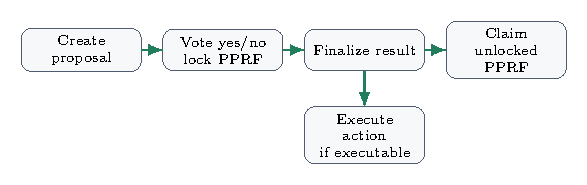
\includegraphics[width=\columnwidth]{governance-flow.pdf}
    \caption{PPRF governance lifecycle. Voting locks funds; finalization determines result; executable proposals may mutate protocol state; voters can claim unlocked funds according to proposal state.}
    \label{fig:governance}
\end{figure}

Executable actions may change fee parameters, type enablement, role configuration, direct authority mode, or other governed state. Execution revalidates proposal status, action enablement, vault binding, and business state. This prevents stale or malformed proposals from becoming permanent privileges.

\section{Agentic Interface}

PaperProof Copilot is a browser-side protocol guide, not an autonomous wallet. It combines a global protocol prompt, page-specific prompt, dynamic page data, recent conversation history, and the user's current question. It can explain an artifact, summarize a governance page, warn about missing balances, clarify whether funds are still locked, and help the user understand what a wallet transaction is likely to do.

\begin{figure}[!t]
    \centering
    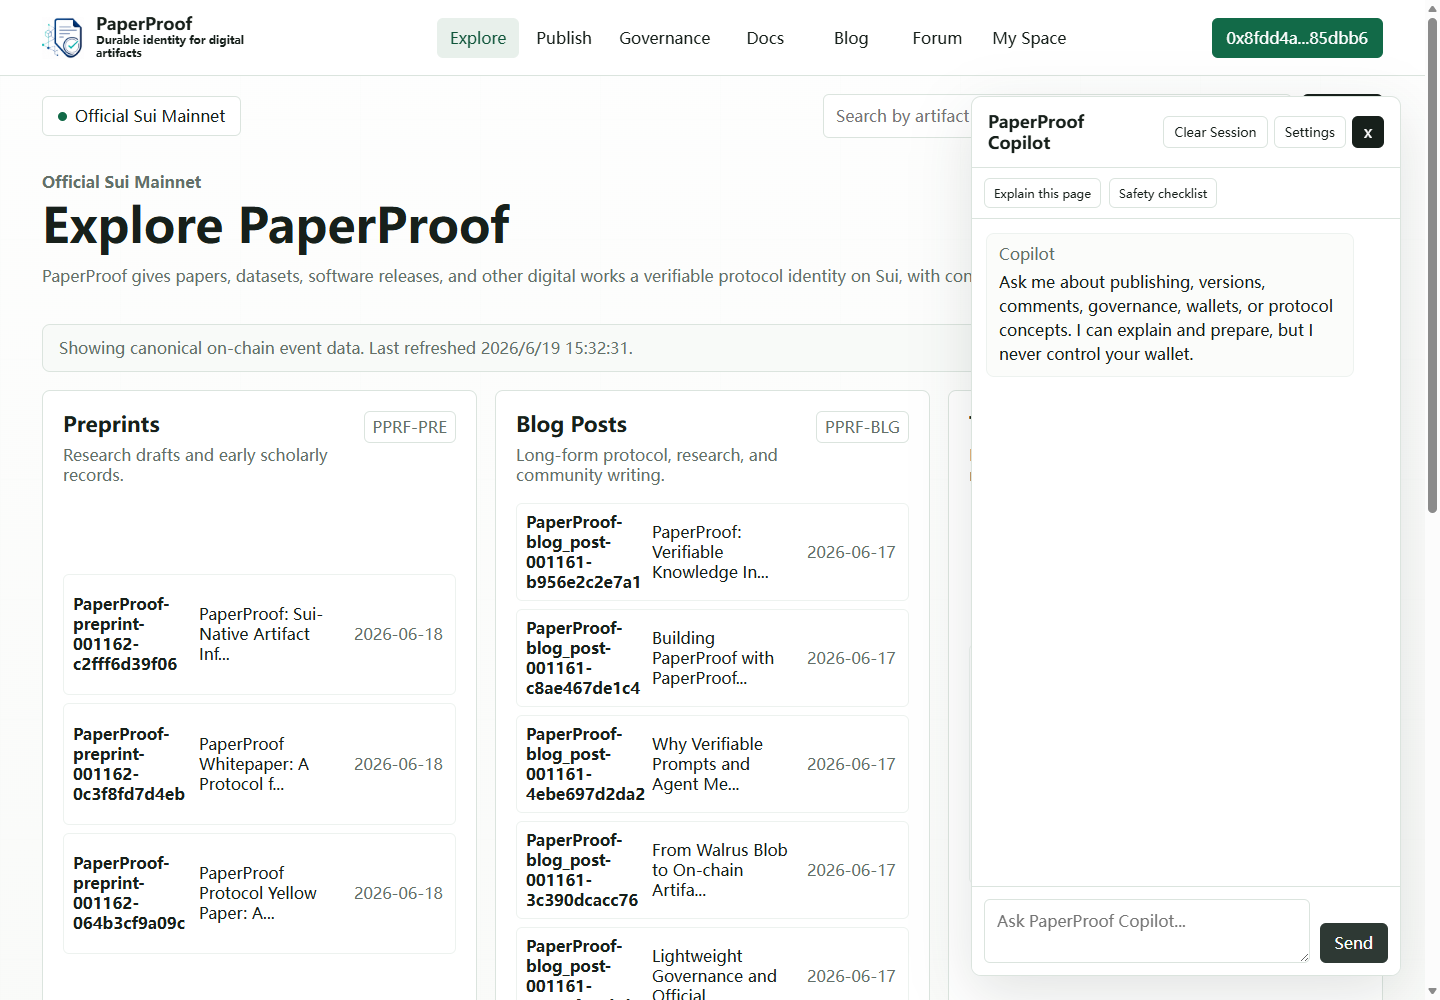
\includegraphics[width=\columnwidth]{copilot-open.png}
    \caption{PaperProof Copilot operates as a browser-side protocol guide. It can read page state and protocol-native prompts, but it remains outside the wallet authorization boundary.}
    \label{fig:copilot_open}
\end{figure}

The safety boundary is explicit. Copilot cannot sign, cannot approve, cannot access seed phrases, and should not ask users for private keys. It prepares understanding; the wallet controls authorization. This pattern is important for Agentic Web systems: AI can become more useful when it reads structured Sui objects and Walrus-backed content, but authority should remain with object permissions and human-approved signatures.

\begin{figure}[!t]
    \centering
    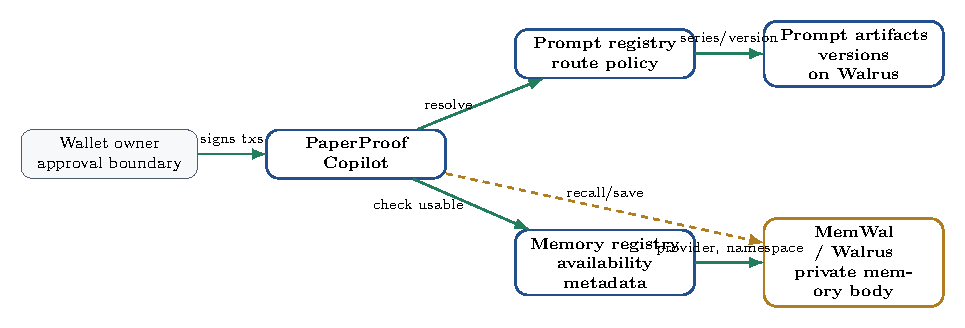
\includegraphics[width=\columnwidth]{agentic-memory-architecture.pdf}
    \caption{Agentic interface architecture. Public registries select official prompt artifacts and memory capability metadata; private memory bodies remain in MemWal/Walrus and are accessed only through user-authorized client flows.}
    \label{fig:agentic_memory}
\end{figure}

\subsection{Agent-Readable State}

PaperProof is useful to agents because it does not present artifacts only as unstructured pages. Artifact type, version lineage, content references, proposal state, voting records, comment trees, and manifest metadata are structured. A model can summarize the current page, explain the meaning of a proposal, compare versions, warn that a provider failed, or describe why a claim is not yet available.

The important design point is that the agent reads protocol state through the same typed surfaces as the application. It is not given hidden authority. This makes the agent a guide over public and wallet-visible facts rather than a privileged backend.

\subsection{Protocol-Native Prompts}

Copilot prompts are treated as artifacts rather than as invisible application constants. The official prompt registry maps an application route to a PaperProof artifact series and either a latest-version or pinned-version policy. The referenced prompt package is stored through the same artifact and Walrus path as other durable content. This makes the prompt layer auditable and replaceable without requiring every static-website deployment to be the final authority on agent behavior.

This design is intentionally modest. The registry does not evaluate prompt quality, does not make model-output guarantees, and does not give the agent additional permissions. It supplies a verifiable coordinate for the instructions an official application intends to use.

\subsection{Wallet-Linked Memory}

Persistent agent memory creates a different trust problem from public artifact prompts. A user's language preference, answer style, current tasks, or recent focus topics can be useful to a Copilot, but these records should not be published directly into public chain state. PaperProof therefore separates memory capability metadata from memory body content. The memory registry records owner, app, provider, namespace, descriptor artifact, version policy, availability, user-enabled state, and deletion tombstone. The private memory body remains in MemWal and Walrus.

\begin{table}[!t]
\caption{Agentic state separation in PaperProof.}
\label{tab:agentic_state}
\centering
\begin{tabularx}{\columnwidth}{p{0.28\columnwidth}X}
\toprule
\textbf{Layer} & \textbf{Role} \\
\midrule
Prompt artifact & Public, versioned instruction package for an app route. \\
Prompt registry & Governed route-to-series/version selector. \\
Memory registry & Public capability metadata and availability state. \\
MemWal memory & Private user memory body and recall/save operations. \\
Wallet & Authorization boundary for chain actions and local access setup. \\
\bottomrule
\end{tabularx}
\end{table}

The registry model also supports management without heavy governance over every memory update. A user may create, disable, or delete their own official memory entry. An operator bound through the governance vault may mark a memory capability unavailable or adjust the descriptor version policy. Deletion is a chain-level tombstone and active-entry release; it does not imply erasure of external Walrus or MemWal blobs.

\subsection{Human-Approved Workflows}

An agentic PaperProof workflow can prepare actions but should not complete them without explicit user approval. For example, Copilot may explain that voting will lock a certain amount of \pprf{}, that funds can be claimed only after finalization, or that extending a non-owned Walrus blob requires shared-blob semantics. The transaction itself is still built through the SDK and approved by the wallet or signer. This pattern keeps AI assistance composable with Sui's object permission model instead of bypassing it.

\section{Implementation and Release Trajectory}

The intended formal release state of PaperProof includes:

\begin{itemize}
    \item Sui mainnet contracts for artifact publishing, comments, likes, governance, fees, and deployment manifests.
    \item Protocol-native prompt and memory registries bound to the governance vault for official Copilot capabilities.
    \item Walrus-backed content flows and a static official application deployable through Walrus Sites.
    \item A TypeScript SDK published to npm for browser and Node.js integration.
    \item A Python SDK published to PyPI for scripting, analytics, export, and notebooks.
    \item A Rust SDK published to crates.io for indexers and backend services.
    \item Optional mainnet read/write scripts, fuzzy tests, examples, and deployment drift checks.
    \item A Sui Prover formal-verification baseline for the four core
    project-side logic modules: publishing, comments, governance, and
    governance voting.
    \item A submission/documentation hub that links contracts, SDKs, application code, slides, deployment evidence, and papers.
\end{itemize}

This implementation posture is unusual for a small protocol but central to PaperProof's claim. The protocol is not merely a contract and a demo. It is a system intended to be used by application developers, data users, indexer builders, and agentic workflow designers.

The paper intentionally describes the formal-release architecture rather than a transient development snapshot. Individual module names, package IDs, and frontend details may change before final public launch, but the architectural commitments are stable: Sui holds official object state, Walrus holds large content and static application surfaces, SDKs expose typed operations, manifests track deployments, and indexers consume canonical events under explicit drift checks.

\subsection{Deployment Manifest Practice}

The deployment manifest is a small but important operational artifact. It records the current network, package bindings, root object, shared object IDs, important type strings, and package version information. It is designed to be read by SDKs, frontends, scripts, and indexers. A manifest lets the protocol upgrade without making every downstream application edit source constants by hand.

This does not remove the need for semantic versioning. If the contract changes event schemas or transaction signatures, SDKs must change. The manifest solves the narrower but common problem of binding discovery. It gives integrators a source of truth for where the current deployment lives and gives drift checkers a way to fail closed when on-chain state does not match the declared deployment.

\subsection{Static Application Deployment}

The official application is designed as a static site because a protocol for durable artifacts should not require a complex server to remain intelligible. A static frontend can query chain state, read Walrus content, load manifests, and build wallet transactions without owning the truth of the protocol. Walrus Sites further strengthens this model by making the application itself part of the same durable content ecosystem.

This does not mean every future PaperProof application must be static. Search-heavy portals, institutional dashboards, enterprise indexers, mobile apps, and community forums may run their own servers. The point is that the base protocol does not depend on one privileged backend to define what was published.

\subsection{Testing Strategy}

PaperProof's testing strategy has three layers. Unit and builder tests validate local rules: input normalization, object ID validation, event parsing, transaction construction, and error boundaries. Mock provider tests validate behavior under missing data, provider failure, pagination, and partial responses. Optional integration tests exercise real Sui and Walrus behavior when explicitly enabled.

Mainnet write tests are useful but must be opt-in. They spend gas, may lock governance funds, may move owned blobs, and may create permanent public artifacts. The project therefore separates local tests, read-only network tests, and write-heavy mainnet scripts. This separation allows CI to remain safe while still giving maintainers a way to validate the full protocol path before releases.

Formal verification is used as complementary evidence rather than as a claim
that every integration path is proven. The current proof baseline covers the
four core project-side logic modules and documents remaining limitations that
come from prover scope, framework modeling, and off-chain integration. This is
appropriate for PaperProof's architecture: Move specifications can strengthen
object and state-transition invariants, while SDK tests, indexer replay, and
mainnet read/write harnesses still carry the cross-system burden involving
providers, wallets, Walrus gateways, caches, and browsers.

\section{Evaluation}

PaperProof should be evaluated as a deployed artifact infrastructure system. The relevant questions are not only throughput or gas cost, but whether the system realizes its trust boundaries and developer surfaces.

\subsection{Functional Coverage}

The implemented system supports publishing, adding versions, comments, blob-backed comments, likes and unlikes, governance proposals, voting, claims, protocol-native prompt resolution, memory capability registration, content read/write/verify/extend/transfer, deployment verification, event parsing, query helpers, and watch APIs. Tests include unit validation, fuzzy validation, builder tests, event parsing, provider behavior, examples, optional mainnet scripts, and indexer behavior.

Functional coverage should be judged at the workflow level rather than only by counting Move functions. A user-facing publish flow requires content preparation, validation, content storage, transaction construction, wallet signing, execution result parsing, series ID extraction, event verification, and query readback. A governance vote requires coin selection, amount normalization, proposal state reading, transaction execution, locked-fund tracking, and later claim support. PaperProof's SDKs are designed to cover these whole workflows.

\subsection{Integration Evidence}

Mainnet integration tests and examples exercise real Sui and Walrus paths when explicitly enabled. These tests are intentionally opt-in because they may spend gas or move assets. The project also distinguishes read-only verification from write-heavy tests so CI remains safe.

The most valuable integration evidence is not a single successful transaction. It is repeated coverage across independent flows: artifact creation, version addition, comments, blob comments, like/unlike, proposal creation, voting, finalization, claim, prompt registration and resolution, memory create/update/delete, content write/read/verify/extend/transfer, query pagination, and indexer backfill. This variety helps reveal argument ordering mistakes, object ownership assumptions, provider page limits, event parsing errors, and result-normalization gaps.

The project also uses PaperProof to publish artifacts that demonstrate the
protocol itself. A Sui Overflow historical winner dataset is published as a
Dataset artifact, and the PaperProof Skill package is published as a Software
Release artifact. These are not synthetic examples: they exercise Walrus
packaging, content hashes, typed metadata, artifact codes, version records,
lookup APIs, and official application rendering.

\begin{figure}[!t]
    \centering
    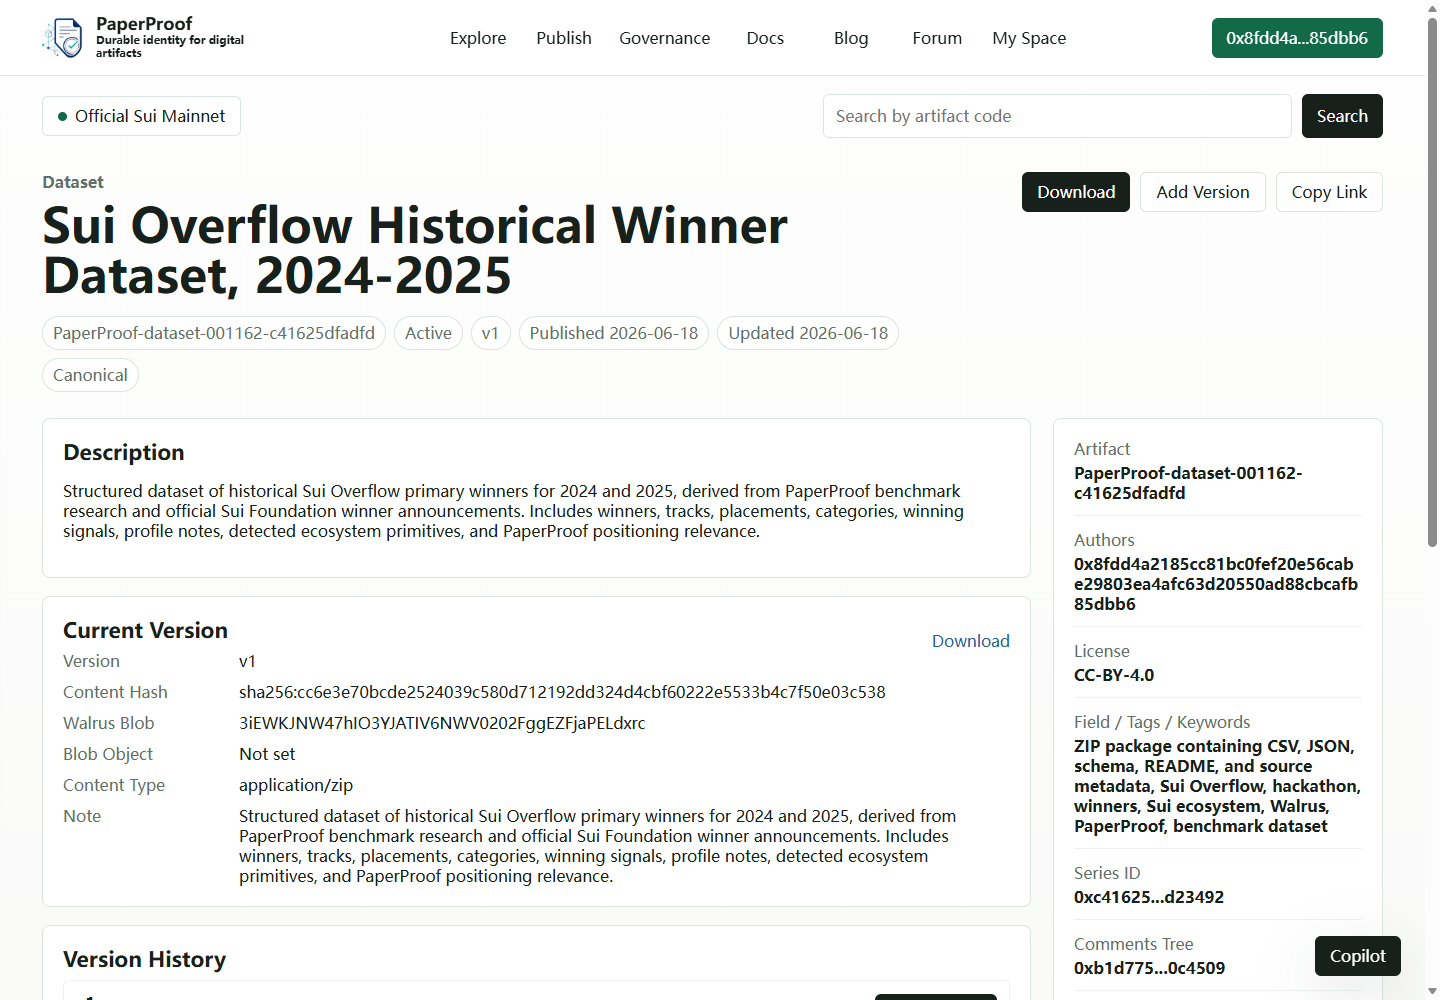
\includegraphics[width=\columnwidth]{dataset-detail.png}
    \caption{A PaperProof Dataset artifact containing Sui Overflow historical winner data. The artifact demonstrates structured dataset publication and lookup through the same protocol path used by papers and software releases.}
    \label{fig:dataset_detail}
\end{figure}

\subsection{Failure-Mode Evaluation}

PaperProof should be evaluated under failure, not only under happy paths. Example failures include invalid object IDs, disabled artifact types, stale deployment manifests, provider timeouts, GraphQL page limits, missing comments objects, old package events, non-shared blob extension attempts, insufficient gas, insufficient \pprf{}, wallet rejection, aborted Move calls, and partially completed content workflows.

A mature SDK should turn these into structured outcomes. Some should fail before signing. Some should fail at dry run. Some should produce transaction execution errors with abort explanations. Some should produce degraded read states rather than empty views. A protocol SDK is reliable when developers can understand and handle these cases without reading raw provider internals.

\subsection{Developer Adoption Readiness}

The publication of three SDKs does not prove adoption, but it demonstrates integration readiness. A third-party developer can use the TypeScript SDK for a static frontend, the Python SDK for analytics and scripts, and the Rust SDK for high-performance indexing. This reduces the risk that the protocol remains accessible only to its original author.

\subsection{Protocol Success Criteria}

The central evaluation target is whether a third party can reconstruct the protocol view without private coordination with PaperProof Labs. A successful implementation should let a developer install an SDK, load the active deployment manifest, query recent artifacts, verify an artifact's content reference, inspect its official comments and likes, follow governance history, and build a transaction for a new interaction. An indexer should be able to backfill events, persist its cursor, reject non-canonical events, resume from failure, and expose derived views without relying on the official frontend.

For users, the success criterion is simpler: within minutes they should understand what an artifact is, retrieve its content, see its versions, read or post comments, vote when appropriate, and avoid signing unclear transactions. The system therefore treats documentation, SDK ergonomics, frontend prompts, and Copilot guidance as part of protocol usability rather than as marketing material.

\subsection{Cost and Performance Expectations}

PaperProof is not designed to put large content on chain. The expected cost profile is many small Sui transactions for state and interaction, plus Walrus storage operations for content. This matches the artifact lifecycle: publishing and versioning are relatively infrequent, while comments, likes, queries, and governance views may be more frequent. The system benefits from Sui's low transaction cost and parallel object execution, while indexers benefit from checkpoint-based ingestion and database sinks.

Future empirical evaluation should report transaction costs for representative publish, add-version, comment, like, vote, claim, prompt registration, memory registration, and content-maintenance flows; storage cost for representative content sizes; indexer backfill throughput; checkpoint lag under tail mode; and frontend query latency under provider failures. These measurements are intentionally separated because a durable artifact protocol should not optimize only one path at the expense of usability or recoverability.

\subsection{Indexing Evaluation}

For indexers, the main performance questions are backfill throughput, tail latency, restart safety, database write latency, memory stability, and rejection accuracy. A high-throughput indexer that accepts wrong events is not useful. A correct indexer that cannot resume safely is not operationally credible. The Rust SDK therefore treats cursor stores, event IDs, database sinks, and drift hard-fail policy as evaluation targets rather than implementation details.

The expected indexer workflow is reproducible: start from a manifest, backfill a checkpoint or event range, apply canonical filters, write accepted events and derived records, record rejected events, persist cursor state, restart, and continue tailing without duplicate domain effects. This workflow should be tested against both empty ranges and active mainnet ranges.

\section{Limitations and Risks}

PaperProof does not solve content quality, legal compliance, plagiarism, academic review, or long-term social governance by itself. Applications and communities must still interpret artifacts.

Walrus storage is durable infrastructure, but content lifecycle still requires renewal, funding, and policy. The SDK can make extension and verification easier, but it cannot eliminate storage economics.

Governance introduces token concentration and participation risks. A vote is a protocol event, not a perfect measure of legitimacy. The protocol should continue to document vote semantics, locked funds, claims, and execution boundaries clearly.

Indexers can still make mistakes if they ignore official object bindings or trust incomplete event providers. This is why deployment manifests, canonical filters, and provider safeguards are part of the SDK design.

The Copilot layer must remain careful. It should explain and guide, not overstate certainty or pressure users into signing. Protocol-native prompts improve auditability but do not eliminate model error. Wallet-linked memory improves continuity but creates privacy and dependency risks if relayers, browsers, or memory providers are misconfigured. The protocol benefits from agent-readable structure only if human authorization and memory boundaries remain clear.

The current memory boundary should not be overstated as complete confidentiality
infrastructure. Keeping memory bodies outside PaperProof Move objects reduces
public exposure, but provider, browser, relay, and storage policy still matter.
A future direction is selective-access protection through a privacy layer such
as Seal. Such integration could strengthen encrypted memory sharing or
cross-agent access control, but it is not required to interpret the current
registry semantics.

\subsection{Protocol Scope Limits}

PaperProof records protocol commitments; it does not certify the truth of content. A fraudulent dataset can still be published. A low-quality preprint can still have a stable artifact identity. A misleading blog post can still be durable. The protocol makes commitments visible and verifiable; it does not replace review, moderation, reputation, or law.

This limitation is not a defect but a boundary. If the protocol tried to decide content truth, it would become a governance-heavy editorial platform. PaperProof instead supplies a common substrate on which different communities can build their own evaluation and moderation systems.

\subsection{Upgrade and Compatibility Risks}

Upgradeability is useful during early protocol development, but it creates compatibility risk. If package IDs, object layouts, event schemas, or execution paths change, downstream applications need accurate manifests and sometimes SDK upgrades. A stale client may show incomplete history or fail to build correct transactions.

PaperProof mitigates this risk with deployment manifests and drift checks, but it cannot eliminate the social requirement that maintainers publish accurate deployment information. Long-term maturity will require clear release processes, versioned schemas, and compatibility documentation.

\subsection{Economic and Governance Risks}

The protocol's economic model must balance spam resistance, accessibility, storage maintenance, and governance sustainability. Fees that are too low may invite spam. Fees that are too high may suppress useful publication. PPRF governance can guide parameters, but token voting introduces its own risks: apathy, concentration, bribery, or governance capture.

The current design therefore treats governance as an auditable mechanism, not as a guarantee of wisdom. Applications should show proposal payloads, vote totals, locked funds, execution status, and claim state so users can reason about governance decisions.

\subsection{Agentic Risks}

Agentic interfaces can improve comprehension, but they can also produce confident errors. A Copilot may misunderstand a proposal, summarize partial data, or fail to notice that a provider degraded. PaperProof reduces this risk by feeding structured page data and protocol prompts to the agent, but the application must still present wallet prompts, raw transaction context, and explicit user approval.

The safest role for an agent is explanatory and preparatory. It can help the user understand a workflow, identify likely risks, and prepare questions. It should not become the authority for whether a transaction is safe.

\section{Related Work}

PaperProof sits at the intersection of decentralized storage, blockchain-based provenance, scholarly communication infrastructure, object-centric smart-contract systems, and developer-facing protocol SDKs.

\subsection{Decentralized Storage and Content Addressing}

IPFS established a widely used content-addressed model for naming and retrieving data independently of a particular host location \cite{benet2014ipfs}. Filecoin adds an incentive layer for decentralized storage markets \cite{protocol_labs2017filecoin}. Arweave proposes an economic model for long-term information permanence \cite{williams2023arweave}. Walrus provides an efficient decentralized storage layer and static-site deployment surface in the Sui ecosystem \cite{danezis2025walrus,walrus_docs}. PaperProof does not compete with these systems as a general storage network. Instead, it uses storage references as one component of a richer artifact identity. The protocol asks which artifact series, version, metadata, comments tree, likes book, proposal, and event stream should be associated with stored content.

\subsection{Blockchain Provenance and Scholarly Communication}

Blockchain provenance work shows the value of tamper-evident records for trust-sensitive systems \cite{xu2019blockchain}. In scholarly communication, prior proposals explored smart papers and smart informetrics \cite{hoffman2019scholarly}, blockchain-supported open peer review \cite{tenorio2021decentralizing}, cooperative scholarly communication platforms \cite{stojmenova2019publish}, and distributed-ledger support for open science and academic publishing \cite{janowicz2018prospects}. DeSci literature further frames decentralization as a set of shared values for research infrastructure rather than as a single technical mechanism \cite{weidener2024desci,hoffman2020decentralization}. PaperProof is aligned with this direction but changes the unit of abstraction from ``paper'' or ``review'' to ``artifact series.'' This allows the same protocol surface to handle preprints, datasets, software releases, technical reports, blog posts, and generic files.

\subsection{Object-Centric Smart Contracts}

Sui's object-centric model makes protocol identity and relationship binding a first-class design option \cite{mysten2022sui,welc2023sui_move,sui_docs}. Move's resource abstraction was designed to represent scarce digital assets with safety properties that are difficult to express in unstructured key-value contract storage \cite{blackshear2020move}. PaperProof relies on these properties to model artifact series, type indexes, official interaction objects, governance vaults, and fee managers as protocol objects rather than as application-side records.

\subsection{PaperProof's Distinction}

The main distinction is that PaperProof combines storage references, object-bound protocol identity, typed version history, official interactions, governance, SDKs, deployment manifests, and indexer primitives in one artifact infrastructure layer. A storage network alone does not define official comments or artifact types. A preprint server alone is usually an application authority. A provenance log alone does not provide SDK-level transaction builders, typed views, watch APIs, or checkpoint indexer support. PaperProof's contribution is the integration boundary: it defines enough protocol structure for independent applications to reconstruct artifact state while leaving social judgment, search ranking, moderation, and presentation to higher layers.

\section{Conclusion}

PaperProof argues that important digital works need more than storage links and application pages. They need durable protocol identities, typed version histories, verifiable content commitments, official interaction objects, governance-aware parameters, and event streams that can be consumed by systems not present at publication time.

By combining Sui object state with Walrus content storage, PaperProof makes artifacts durable without pretending that every social or editorial judgment belongs on-chain. By shipping role-specific SDKs and indexer tools, it treats developer experience as part of protocol design. By introducing a human-approved Copilot interface, it shows how agentic workflows can interpret Sui-native artifact state without controlling user authority.

More broadly, PaperProof treats artifacts, prompts, memory descriptors, reports,
datasets, logs, and software releases as points on the same design spectrum:
durable knowledge objects whose public commitments can be resolved across
applications and over time. This is the main systems claim of the project.

The result is not a replacement for archives, repositories, social platforms, or storage networks. It is a protocol layer beneath and beside them: a durable coordinate system for artifacts that should remain verifiable, discussable, governable, and readable by future applications.

\bibliographystyle{ieeetr}
\bibliography{Ref}

\end{document}
